

\tikzset{every picture/.style={line width=0.75pt}} %set default line width to 0.75pt        

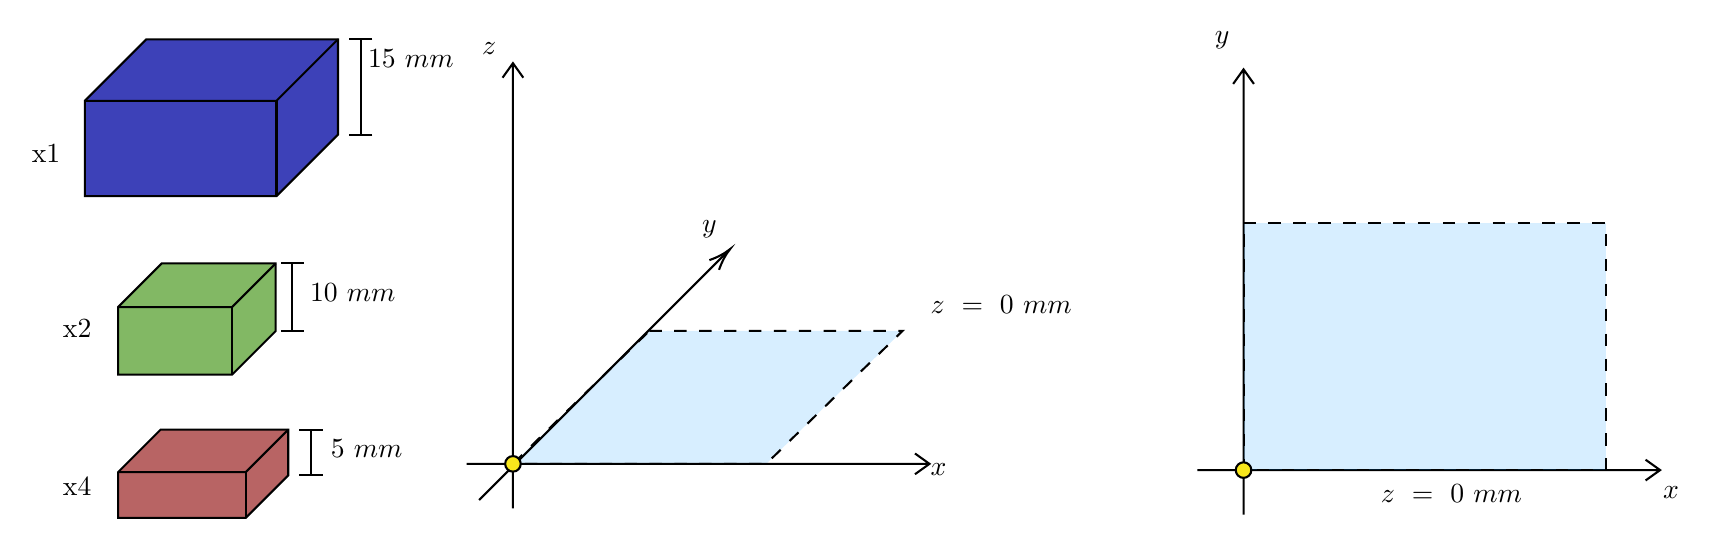
\begin{tikzpicture}[x=0.75pt,y=0.75pt,yscale=-1,xscale=1]
%uncomment if require: \path (0,285); %set diagram left start at 0, and has height of 285

%Shape: Parallelogram [id:dp9478669737271833] 
\draw  [fill={rgb, 255:red, 17; green, 154; blue, 255 }  ,fill opacity=0.17 ][dash pattern={on 4.5pt off 4.5pt}] (311,164) -- (433,164) -- (367.3,228.05) -- (245.3,228.05) -- cycle ;
%Shape: Axis 2D [id:dp9053839130374074] 
\draw  (223,228.05) -- (446,228.05)(245.3,35) -- (245.3,249.5) (439,223.05) -- (446,228.05) -- (439,233.05) (240.3,42) -- (245.3,35) -- (250.3,42)  ;
%Straight Lines [id:da1625430749081903] 
\draw    (229,245.5) -- (348.59,125.91) ;
\draw [shift={(350,124.5)}, rotate = 135] [color={rgb, 255:red, 0; green, 0; blue, 0 }  ][line width=0.75]    (10.93,-3.29) .. controls (6.95,-1.4) and (3.31,-0.3) .. (0,0) .. controls (3.31,0.3) and (6.95,1.4) .. (10.93,3.29)   ;
%Shape: Circle [id:dp5639312612319123] 
\draw  [fill={rgb, 255:red, 248; green, 231; blue, 28 }  ,fill opacity=1 ] (241.55,228.05) .. controls (241.55,225.98) and (243.23,224.3) .. (245.3,224.3) .. controls (247.37,224.3) and (249.05,225.98) .. (249.05,228.05) .. controls (249.05,230.12) and (247.37,231.8) .. (245.3,231.8) .. controls (243.23,231.8) and (241.55,230.12) .. (241.55,228.05) -- cycle ;
%Shape: Axis 2D [id:dp7452949972997148] 
\draw  (575,231.05) -- (798,231.05)(597.3,38) -- (597.3,252.5) (791,226.05) -- (798,231.05) -- (791,236.05) (592.3,45) -- (597.3,38) -- (602.3,45)  ;
%Shape: Rectangle [id:dp3032130370245537] 
\draw  [fill={rgb, 255:red, 17; green, 154; blue, 255 }  ,fill opacity=0.17 ][dash pattern={on 4.5pt off 4.5pt}] (597.3,112) -- (772,112) -- (772,231.05) -- (597.3,231.05) -- cycle ;
%Shape: Circle [id:dp4579792139014013] 
\draw  [fill={rgb, 255:red, 248; green, 231; blue, 28 }  ,fill opacity=1 ] (593.55,231.05) .. controls (593.55,228.98) and (595.23,227.3) .. (597.3,227.3) .. controls (599.37,227.3) and (601.05,228.98) .. (601.05,231.05) .. controls (601.05,233.12) and (599.37,234.8) .. (597.3,234.8) .. controls (595.23,234.8) and (593.55,233.12) .. (593.55,231.05) -- cycle ;
%Shape: Cube [id:dp562537314193528] 
\draw  [fill={rgb, 255:red, 184; green, 100; blue, 100 }  ,fill opacity=1 ] (55.05,232.05) -- (75.55,211.55) -- (137.05,211.55) -- (137.05,233.55) -- (116.55,254.05) -- (55.05,254.05) -- cycle ; \draw   (137.05,211.55) -- (116.55,232.05) -- (55.05,232.05) ; \draw   (116.55,232.05) -- (116.55,254.05) ;
%Shape: Cube [id:dp21248572948665245] 
\draw  [fill={rgb, 255:red, 130; green, 184; blue, 100 }  ,fill opacity=1 ] (55.05,152.5) -- (76.05,131.5) -- (131,131.5) -- (131,164.05) -- (110,185.05) -- (55.05,185.05) -- cycle ; \draw   (131,131.5) -- (110,152.5) -- (55.05,152.5) ; \draw   (110,152.5) -- (110,185.05) ;
%Shape: Cube [id:dp5751910582035913] 
\draw  [fill={rgb, 255:red, 61; green, 65; blue, 184 }  ,fill opacity=1 ] (39.05,53.13) -- (68.68,23.5) -- (161,23.5) -- (161,69.42) -- (131.37,99.05) -- (39.05,99.05) -- cycle ; \draw   (161,23.5) -- (131.37,53.13) -- (39.05,53.13) ; \draw   (131.37,53.13) -- (131.37,99.05) ;
%Straight Lines [id:da42543949918671464] 
\draw    (148.05,211.55) -- (148.05,233.55) ;
\draw [shift={(148.05,233.55)}, rotate = 270] [color={rgb, 255:red, 0; green, 0; blue, 0 }  ][line width=0.75]    (0,5.59) -- (0,-5.59)   ;
\draw [shift={(148.05,211.55)}, rotate = 270] [color={rgb, 255:red, 0; green, 0; blue, 0 }  ][line width=0.75]    (0,5.59) -- (0,-5.59)   ;
%Straight Lines [id:da6252654506223498] 
\draw    (139,131.5) -- (139,164.05) ;
\draw [shift={(139,164.05)}, rotate = 270] [color={rgb, 255:red, 0; green, 0; blue, 0 }  ][line width=0.75]    (0,5.59) -- (0,-5.59)   ;
\draw [shift={(139,131.5)}, rotate = 270] [color={rgb, 255:red, 0; green, 0; blue, 0 }  ][line width=0.75]    (0,5.59) -- (0,-5.59)   ;
%Straight Lines [id:da850203723421372] 
\draw    (172,23.5) -- (172,69.42) ;
\draw [shift={(172,69.42)}, rotate = 270] [color={rgb, 255:red, 0; green, 0; blue, 0 }  ][line width=0.75]    (0,5.59) -- (0,-5.59)   ;
\draw [shift={(172,23.5)}, rotate = 270] [color={rgb, 255:red, 0; green, 0; blue, 0 }  ][line width=0.75]    (0,5.59) -- (0,-5.59)   ;

% Text Node
\draw (445,145.4) node [anchor=north west][inner sep=0.75pt]    {$z\ =\ 0\ mm$};
% Text Node
\draw (335,109.4) node [anchor=north west][inner sep=0.75pt]    {$y$};
% Text Node
\draw (445,226.4) node [anchor=north west][inner sep=0.75pt]    {$x$};
% Text Node
\draw (229,23.4) node [anchor=north west][inner sep=0.75pt]    {$z$};
% Text Node
\draw (798,237.4) node [anchor=north west][inner sep=0.75pt]    {$x$};
% Text Node
\draw (582,18.4) node [anchor=north west][inner sep=0.75pt]    {$y$};
% Text Node
\draw (662,236.4) node [anchor=north west][inner sep=0.75pt]    {$z\ =\ 0\ mm$};
% Text Node
\draw (27,157) node [anchor=north west][inner sep=0.75pt]   [align=left] {x2};
% Text Node
\draw (12,73) node [anchor=north west][inner sep=0.75pt]   [align=left] {x1};
% Text Node
\draw (27,233) node [anchor=north west][inner sep=0.75pt]   [align=left] {x4};
% Text Node
\draw (156.05,214.95) node [anchor=north west][inner sep=0.75pt]    {$5\ mm$};
% Text Node
\draw (146.05,139.95) node [anchor=north west][inner sep=0.75pt]    {$10\ mm$};
% Text Node
\draw (174,26.9) node [anchor=north west][inner sep=0.75pt]    {$15\ mm$};


\end{tikzpicture}
